
\documentclass{vgtc}                          % final (conference style)
%\documentclass[review]{vgtc}                 % review
%\documentclass[widereview]{vgtc}             % wide-spaced review
%\documentclass[preprint]{vgtc}               % preprint
%\documentclass[electronic]{vgtc}             % electronic version

%% Uncomment one of the lines above depending on where your paper is
%% in the conference process. ``review'' and ``widereview'' are for review
%% submission, ``preprint'' is for pre-publication, and the final version
%% doesn't use a specific qualifier. Further, ``electronic'' includes
%% hyperreferences for more convenient online viewing.

%% Please use one of the ``review'' options in combination with the
%% assigned online id (see below) ONLY if your paper uses a double blind
%% review process. Some conferences, like IEEE Vis and InfoVis, have NOT
%% in the past.

%% Figures should be in CMYK or Grey scale format, otherwise, colour 
%% shifting may occur during the printing process.

%% These few lines make a distinction between latex and pdflatex calls and they
%% bring in essential packages for graphics and font handling.
%% Note that due to the \DeclareGraphicsExtensions{} call it is no longer necessary
%% to provide the the path and extension of a graphics file:
%% \includegraphics{diamondrule} is completely sufficient.
%%
\ifpdf%                                % if we use pdflatex
  \pdfoutput=1\relax                   % create PDFs from pdfLaTeX
  \pdfcompresslevel=9                  % PDF Compression
  \pdfoptionpdfminorversion=7          % create PDF 1.7
  \ExecuteOptions{pdftex}
  \usepackage{graphicx}                % allow us to embed graphics files
  \DeclareGraphicsExtensions{.pdf,.png,.jpg,.jpeg} % for pdflatex we expect .pdf, .png, or .jpg files
\else%                                 % else we use pure latex
  \ExecuteOptions{dvips}
  \usepackage{graphicx}                % allow us to embed graphics files
  \DeclareGraphicsExtensions{.eps}     % for pure latex we expect eps files
\fi%

%% it is recomended to use ``\autoref{sec:bla}'' instead of ``Fig.~\ref{sec:bla}''
\graphicspath{{figures/}{pictures/}{images/}{./}} % where to search for the images

\usepackage{microtype}                 % use micro-typography (slightly more compact, better to read)
\PassOptionsToPackage{warn}{textcomp}  % to address font issues with \textrightarrow
\usepackage{textcomp}                  % use better special symbols
\usepackage{mathptmx}                  % use matching math font
\usepackage{times}                     % we use Times as the main font
\renewcommand*\ttdefault{txtt}         % a nicer typewriter font
\usepackage{cite}                      % needed to automatically sort the references
\usepackage{tabu}                      % only used for the table example
\usepackage{booktabs}                  % only used for the table example
%% We encourage the use of mathptmx for consistent usage of times font
%% throughout the proceedings. However, if you encounter conflicts
%% with other math-related packages, you may want to disable it.

%% wes 8/2021 additions
\usepackage{comment}    % wes 8/2021
\usepackage{color}      % wes 8/2021
\usepackage{listings}   % wes 8/2021

%% Shun 9/2024 additions
\usepackage{placeins}   % for \FloatBarrier
\usepackage{afterpage} % For \afterpage{\clearpage}
\usepackage{amsmath}
\usepackage[labelfont=bf]{caption} % For make the figure title "Figure 2. " bold
\usepackage{appendix}
\usepackage{graphicx}    % For including graphics
\usepackage{caption}     % For customizing captions
\usepackage{subcaption}  % For creating subfigures
\usepackage{url} 
\usepackage[]{algorithm2e} % For pseudo code
% wes: for code formatting/coloring
\definecolor{codegreen}{rgb}{0,0.6,0}
\definecolor{codegray}{rgb}{0.5,0.5,0.5}
\definecolor{codepurple}{rgb}{0.58,0,0.82}
\definecolor{backcolour}{rgb}{0.95,0.95,0.92}
\definecolor{codecyan}{rgb}{0.0,0.2,1.0}

% see: https://en.wikibooks.org/wiki/LaTeX/Source_Code_Listings
% set font, size, color style for code listings
\lstdefinestyle{mystyle}{
%    backgroundcolor=\color{backcolour},   
    commentstyle=\textcolor{codegreen},
%    keywordstyle=\color{magenta},    
    keywordstyle=\color{codecyan},
    numberstyle=\tiny\color{codegray},
    stringstyle=\color{codepurple},
    basicstyle=\ttfamily\footnotesize,
    breakatwhitespace=false,    
    breaklines=true,    
    captionpos=b,    
    keepspaces=true,    
    numbers=left,    
    numbersep=2pt,  
    firstnumber=auto,
    numberblanklines=false,
    showspaces=false,
    showstringspaces=false,
    showtabs=false,
    tabsize=2
}
% and then set mystyle to be the default when doing code listings
\lstset{style=mystyle}



%% If you are submitting a paper to a conference for review with a double
%% blind reviewing process, please replace the value ``0'' below with your
%% OnlineID. Otherwise, you may safely leave it at ``0''.
\onlineid{0}

%% declare the category of your paper, only shown in review mode
\vgtccategory{Research}

%% allow for this line if you want the electronic option to work properly
% 8/2021 wes comment out the following line to eliminate build warnings
%\vgtcinsertpkg

%% In preprint mode you may define your own headline.
%\preprinttext{To appear in an IEEE VGTC sponsored conference.}

%% Paper title.

\title{Parallel Ray Tracing \\Term Project, CSC 746, Fall 2024}

%% This is how authors are specified in the conference style

%% Author and Affiliation (single author).
%%\author{Roy G. Biv\thanks{e-mail: roy.g.biv@aol.com}}
%%\affiliation{\scriptsize Allied Widgets Research}

%% Author and Affiliation (multiple authors with single affiliations).
%%\author{Roy G. Biv\thanks{e-mail: roy.g.biv@aol.com} %
%%\and Ed Grimley\thanks{e-mail:ed.grimley@aol.com} %
%%\and Martha Stewart\thanks{e-mail:martha.stewart@marthastewart.com}}
%%\affiliation{\scriptsize Martha Stewart Enterprises \\ Microsoft Research}

%% Author and Affiliation (multiple authors with multiple affiliations)
\author{Shun Usami\thanks{email:susami@sfsu.edu}\\ %
        \scriptsize SFSU}

%% A teaser figure can be included as follows, but is not recommended since
%% the space is now taken up by a full width abstract.
%\teaser{
%  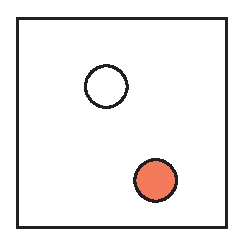
\includegraphics[width=1.5in]{sample.eps}
%  \caption{Lookit! Lookit!}
%}

%% Abstract section.
\abstract{
% Please take a few moments and try to compose an abstract for your homework writeup. It should contain these ideas: what was the problem being studied, what was the approach (what did you implement), what are the results.
% The abstract should describe the basic message of the paper, including: the problem, why your solution should be of interest, some notion that your solution is effective, and a teaser about how it has been evaluated. Cover all of this using between 75 and 150 words. Thus, the abstract is the hardest part to write. Sometimes I try to write it first, but the final version is usually composed of items drawn from the introduction, and then condensed, as the last step of writing the paper.

% describes the focus of the study, the approach, and the primary findings/results (3 or 4 sentences total). Writing tip: it's often the case that the Abstract and Introduction are the last items written in a technical paper, once you know the outcome of the performance study.

This assignment investigates two performance optimization techniques—parallelism and cache utilization—by evaluating the performance of three matrix multiplication (MM) methods: Basic Matrix Multiplication with OpenMP (Basic OMP), Blocked Matrix Multiply with Copy Optimization (BMMCO OMP), and CBLAS, using hardware counters. The implementations were tested across varying matrix sizes (\(128 \times 128\), \(512 \times 512\), and \(2048 \times 2048\)) and thread counts (1, 4, 16, and 64) to assess speedup and efficiency. Results indicate that while Basic OMP scales effectively with increasing thread count, BMMCO OMP exhibits limited scalability for smaller matrices and larger block sizes due to thread underutilization. The BMMCO OMP method significantly reduced L2 and L3 cache accesses, particularly with larger block sizes, resulting in superior performance compared to Basic OMP. These findings suggest that achieving optimal performance requires balancing between increasing cache utilization through larger block sizes and maximizing thread utilization with smaller block sizes.
} % end of abstract

%% ACM Computing Classification System (CCS). 
%% See <http://www.acm.org/class/1998/> for details.
%% The ``\CCScat'' command takes four arguments.

% not needed for CSC 746 Fall 2021
%\CCScatlist{ 
%  \CCScat{K.6.1}{Management of Computing and Information Systems}%
%{Project and People Management}{Life Cycle};
%  \CCScat{K.7.m}{The Computing Profession}{Miscellaneous}{Ethics}
%}

%% Copyright space is enabled by default as required by guidelines.
%% It is disabled by the 'review' option or via the following command:
% \nocopyrightspace

%%%%%%%%%%%%%%%%%%%%%%%%%%%%%%%%%%%%%%%%%%%%%%%%%%%%%%%%%%%%%%%%
%%%%%%%%%%%%%%%%%%%%%% START OF THE PAPER %%%%%%%%%%%%%%%%%%%%%%
%%%%%%%%%%%%%%%%%%%%%%%%%%%%%%%%%%%%%%%%%%%%%%%%%%%%%%%%%%%%%%%%%

\begin{document}

\maketitle
%% The ``\maketitle'' command must be the first command after the
%% ``\begin{document}'' command. It prepares and prints the title block.

%% the only exception to this rule is the \firstsection command
%\firstsection{Introduction}

\section{Introduction}
% consists of 3 short paragraphs consisting of the problem statement, your approach, and a brief summary of the findings/results. Here, short paragraph means 3-4 sentences.

The objective of this study is to evaluate the effectiveness of different parallelization techniques for enhancing computational efficiency and memory bandwidth utilization in matrix-vector multiplication (VMM). The techniques explored include instruction-level parallelism, SIMD instructions, vectorization, multi-threading with OpenMP, and considerations for NUMA architecture. By examining these methods, we aim to understand their respective benefits and limitations in the context of high-performance computing.

We implemented four versions of VMM: a basic serial version as an unoptimized baseline, a highly optimized serial version using the CBLAS library, an automatically vectorized serial version leveraging SIMD instructions, and a parallel version utilizing OpenMP for multi-threading. These implementations provide a comprehensive basis for evaluating the impact of different optimizations on performance. All experiments were conducted on the Perlmutter supercomputer at NERSC, using C++ for implementation. Detailed descriptions of these methods are provided in Section~\ref{sec:methodology}.

The results indicate that the Vectorized implementation achieved four times the performance of the Basic version due to SIMD instructions and performed similarly to CBLAS for larger matrix sizes. However, CBLAS significantly outperformed the Vectorized version for smaller matrices, likely due to techniques like instruction-level parallelism (ILP). The OpenMP implementation, while outperforming CBLAS for larger matrices, had excessive overhead for smaller sizes, making it worse than both CBLAS and even the Vectorized version. Despite outperforming CBLAS for larger sizes, the OpenMP performance was still far from ideal due to memory data layout inefficiencies and limited bandwidth, which acted as bottlenecks.
% For homework writeups, the Introduction section should state the general thrust of the assignment.

% What is the problem being studied? Explain in 2-3 sentences.

% What is the approach for studying the problem? Hint: the approach consists of the program(s) you are writing, so say in 2-3 sentences something about those programs. If you like, it is ok to use a forward reference, and say something like "we present the implementation in \S\ref{sec:implementation}. 

% What are the main results? Say something about the results in 2-3 sentences: what is the nature of your experiment that tests your implementation, and say something about the insights gained. 

\begin{comment}
%% the material that follows is from the generic tech paper skeleton project

The problem we have solved
\begin{itemize}
    \item Concentrate on making this assertion and only this assertion in a succinct set of 1 to 3 paragraphs
    \item A common mistake is to explain too much of the problem context first. Instead, state the problem essentially as a claim, and leave explanations supporting your claim to the next part, “Why it is not already solved.”
\end{itemize}

Why the problem is not already solved or other solutions are ineffective in one or more important ways
\begin{itemize}

\item Your new idea need not solve every problem but it should solve at least one that is not already solved
\item This is the place to provide a succinct description of the problem context giving enough information to support the claim that a problem exists, made in the preceding problem declaration.
  
\end{itemize}

Why our solution is worth considering and why is it effective in some way that others are not

\begin{itemize}
\item A succinct statement of why the reader should care enough to read the rest of the paper.
\item This should include a statement about the characteristics of your solution to the problem which 1) make it a solution, and 2) make it superior to other solutions to the same problem.
\end{itemize}

How the rest of the paper is structured
\begin{itemize}
    \item The short statement below is often all you need, but you should change it when your paper has a different structure, or when more information is required to describe what a given section contains. If it isn’t required then you don’t want to say it here.
\end{itemize}

The rest of this paper first discusses related work in Section 2, and then describes our implementation in Section 3. Section 4 describes how we evaluated our system and presents the results. Section 5 presents our conclusions and describes future work.

\end{comment}
\section{Related Work}
\label{sec:related-work}
Ray tracing has been a cornerstone of photorealistic rendering since its inception, with significant advancements in both algorithms and hardware optimization.

Phong Shading~\cite{Phong1975} introduced a realistic shading model in 1975 that enhanced 3D rendering by approximating light interactions on surfaces. Whitted's Ray Tracing~\cite{Whitted1980} expanded the paradigm in 1980 to incorporate global illumination effects such as reflections, refractions, and shadows, laying the groundwork for modern physically-based rendering techniques.

Subsequent innovations, such as Distributed Ray Tracing~\cite{Cook1984}, addressed issues like aliasing and simulated effects such as motion blur and soft shadows through distributed sampling. The Rendering Equation~\cite{Kajiya1986} unified various rendering approaches under a single mathematical framework in 1986, enabling sophisticated solutions for complex illumination scenarios.

With the advent of GPUs, significant effort has been devoted to optimizing ray tracing for parallel hardware. For example, GPU Ray Traversal Optimization~\cite{Aila2009} in 2009 identified bottlenecks in memory bandwidth and workload distribution, proposing techniques such as persistent threads to enhance performance.

Despite these advancements, achieving real-time ray tracing remains a challenge, especially on general-purpose hardware. Existing methods often encounter limitations such as load imbalance and inefficient utilization of parallel resources, motivating further exploration of parallelization strategies tailored to CPUs.

\section{Implementation}
\label{sec:implementation}
% Put an introductory paragraph here that gives the reader an overview of what's coming. If there are multiple subsections, say in a few words or a sentence something about each subsection.

% include a separate subsection for each of the different implementations. Briefly describe your implementation, and include the use of compact pseudocode as necessary. The focus here should be on conciseness and clarity. Be sure to describe the strategy you used in parallelizing your code. Your example Listings should clearly indicate the OpenMP pragmas you used. 
In this study, we implemented two versions of a ray tracing system: a serial implementation (Serial RT) and a parallel implementation using OpenMP (OpenMP RT). These implementations were designed to explore the performance differences and challenges in parallelizing ray tracing on multi-core CPUs.

\subsection{Ray tracing foundations}
\label{subsec:ray-tracing-foundations}
The objective of this section is to establish the core principles and computational steps underlying the ray tracing process. By defining methods for rendering an image, generating rays, determining ray colors through recursive evaluation, and testing for intersections, we set the groundwork for producing visually accurate, physically plausible images.

This section introduces the essential components of a ray tracing pipeline, from pixel-by-pixel rendering to ray generation, color computation, and intersection handling. The details, supported by pseudo-code and listings, show how rays are cast, how intersections and scattering are computed, and how final colors are accumulated.

\subsubsection{Rendering}
This subsection outlines the process of computing the final image by iterating over each pixel, generating multiple rays per pixel, computing their colors, and averaging the results, as shown in Algorithm \ref{alg:rendering}.

\begin{algorithm}[htbp]
\KwData{image\_height, image\_width, samples\_per\_pixel, max\_recursion\_depth, world}
initialize image\;
\For{$y = 0$ \KwTo $image\_height$}{
    \For{$x = 0$ \KwTo $image\_width$}{
        \For{$i = 0$ \KwTo $samples\_per\_pixel$}{
            $r \gets get\_ray(x, y)$\;
            $image[x, y] \gets image[x, y] + ray\_color(r, max\_recursion\_depth, world)$\;
        }
    }
}
write image\;
\caption{\textbf{Render Image.} Loop structure for rendering an image by averaging multiple samples per pixel.}
\label{alg:rendering}
\end{algorithm}

\FloatBarrier
\subsubsection{Generating Ray}
This subsection details how a ray is constructed from the camera to a specific pixel, incorporating randomness for anti-aliasing and depth-of-field effects, as shown in Listing \ref{listing:get-ray}.

\begin{lstlisting}[caption={\textbf{Generating a ray from the camera to a screen pixel}},label={listing:get-ray}, name=get-ray, float=htbp, style=mystyle,language=C++]
ray get_ray(int i, int j) const {
    auto offset = sample_square();
    auto pixel_sample = pixel00_loc + (i + offset.x()) * pixel_delta_u + (j + offset.y()) * pixel_delta_v;
    auto ray_origin = (defocus_angle <= 0) ? center : defocus_disk_sample();
    auto ray_direction = pixel_sample - ray_origin;
    return ray(ray_origin, ray_direction);
}
\end{lstlisting}

\FloatBarrier
\subsubsection{Computing a ray's color}
This subsection explains the recursive computation of a ray’s color as it interacts with objects, possibly scattering to produce reflections and other effects, or returning a background color if no objects are hit, as shown in Listing \ref{listing:ray-color}.

\begin{lstlisting}[caption={\textbf{Computing a ray's color}},label={listing:ray-color}, name=ray-color, float=htbp, style=mystyle,language=C++]
color ray_color(const ray &r, int depth, const hittable &world) {
    if (depth <= 0) return color(0, 0, 0);
    hit_record rec;
    if (world.hit(r, interval(0.001, infinity), rec)) {
      ray scattered;
      color attenuation;
      if (rec.mat->scatter(r, rec, attenuation, scattered))
        return attenuation * ray_color(scattered, depth - 1, world);
      return color(0, 0, 0);
    }
    return sky_color(r);
}
\end{lstlisting}

\FloatBarrier
\subsubsection{Intersection test with ray and scene}
This subsection describes how the ray is tested against a set of objects to find the closest intersection, enabling accurate shading calculations. This implementation naively iterates over every object in the scene, without employing more advanced acceleration structures such as Bounding Volume Hierarchies\cite{Kay1986}. See Listing \ref{listing:hittable-list}.

\begin{lstlisting}[caption={\textbf{Hittable List Implementation}}, label={listing:hittable-list}, name=hittable-list, float=htbp, style=mystyle, language=C++]
class hittable_list : public hittable {
  std::vector<shared_ptr<hittable>> objects;

  bool hit(const ray &r, interval ray_t, hit_record &rec) const override {
    hit_record temp_rec;
    bool hit_anything = false;
    auto closest_so_far = ray_t.max;

    for (const auto &object : objects) {
      if (object->hit(r, interval(ray_t.min, closest_so_far), temp_rec)) {
        hit_anything = true;
        closest_so_far = temp_rec.t;
        rec = temp_rec;
      }
    }

    return hit_anything;
  }
};
\end{lstlisting}

\subsection{Serial RT}
\label{subsec:serial-rt}
While no standalone serial implementation was created, the OpenMP implementation with a single-thread parameter (\texttt{OMP\_NUM\_THREADS=1}) serves as the baseline for evaluating parallel performance. This approach processes each pixel sequentially, tracing rays from the camera through the scene, computing intersections, and determining the final color for each pixel. Although straightforward, this single-threaded execution lacks the scalability needed for real-time rendering of complex scenes.

\begin{lstlisting}[caption={\textbf{Serial RT:} The baseline implementation computes the color of each pixel by casting multiple rays per pixel (antialiasing) and aggregating their contributions. Each pixel's color is computed independently.}, label={listing:serial-rt}, name=serial-rt, float=htbp, style=mystyle, language=C++]
for (int y = 0; y < height; y++) {
  for (int x = 0; x < width; x++) {
    color pixel_color = color(0, 0, 0);
    for (int s = 0; s < samples_per_pixel; s++) {
      ray r = get_ray(x, y);
      pixel_color += ray_color(r, max_depth, world);
    }
    image[y * image_width + x] += pixel_color;
  }
}
\end{lstlisting}

\FloatBarrier
\subsection{OpenMP RT}
\label{subsec:openmp-rt}
The parallel implementation leverages OpenMP to distribute the computational workload across multiple threads. By parallelizing the per-pixel ray tracing task, we aim to achieve significant performance improvements over the serial version.

\begin{lstlisting}[caption={\textbf{OpenMP RT:} This parallelized implementation uses OpenMP to distribute pixel computations across multiple threads. The \texttt{\#pragma omp parallel for} directive enables efficient workload distribution, with optional loop collapsing (\texttt{collapse(2)}) for combining nested loops. The scheduling policy is configurable at runtime, allowing flexible tuning to balance performance and overhead.}, label={listing:openmp-rt}, name=openmp-rt, float=htbp, style=mystyle, language=C++]
#if OMP_COLLAPSE
#pragma omp parallel for collapse(2) schedule(runtime)
#else
#pragma omp parallel for schedule(runtime)
#endif
for (int y = 0; y < height; y++) {
  for (int x = 0; x < width; x++) {
    color pixel_color = color(0, 0, 0);
    for (int s = 0; s < samples_per_pixel; s++) {
      ray r = get_ray(x, y);
      pixel_color += ray_color(r, max_depth, world);
    }
    image[y * image_width + x] += pixel_color;
  }
}
\end{lstlisting}

\subsubsection{Parallelization Strategy}
The OpenMP implementation focuses on parallelizing the loop that iterates over image pixels. Each thread processes a subset of the pixels independently, taking advantage of the embarrassingly parallel nature of the problem. Two scheduling strategies were implemented and evaluated:

\begin{itemize}
    \item \textbf{Static Scheduling:} Pixels are evenly divided among threads at compile time. This approach is efficient for simple scenes but can lead to load imbalance in complex ones.
    \item \textbf{Dynamic Scheduling:} Pixels are assigned to threads in smaller chunks at runtime, improving load balancing but introducing overhead due to runtime scheduling decisions.
\end{itemize}



\begin{comment}
%% the material that follows is from the generic tech paper skeleton project

\begin{itemize}
    \item Another way to look at this section is as a paper, within a paper, describing your implementation. That viewpoint makes this the introduction to the subordinate paper, which should describe the overall structure of your implementation and how it is designed to address the problem effectively.
\item Then, describe the structure of the rest of this section, and what each subsection describes.
\end{itemize}

How our solution (will | does) work
\begin{itemize}
    \item This is the body of the subordinate paper describing your solution. It may be divided into several subsections as required by the nature of your implementation.
    \item The level of detail about how the solution works is determined by what is appropriate to the type of paper (conference, journal, technical report).
    \item This section can be fairly short for conference papers, fairly long for journal papers, or quite long in technical reports. It all depends on the purpose of the paper and the target audience.
    \item Proposals are necessarily a good deal more vague in this section since you have to convince someone you know enough to have a good chance of building a solution, but that you have not already done so.
\end{itemize}

\end{comment}

\section{Evaluation}

% Provide an introductory paragraph that summarizes what's in this section: a list of runs/experiments intended to test your implementation and ideas. Describe each of these experiments in a few words/a sentence.
In this section, we present the results of our experiments, aimed at evaluating the performance of the matrix multiplication implementations introduced earlier. We conducted tests on the Perlmutter supercomputer to compare the computational throughput (in MFLOP/s) of three matrix multiplication methods: Basic MM (unoptimized) and CBLAS (highly optimized) as performance baselines, and Blocked Matrix Multiplication with Copy Optimization (BMMCO) to analyze the impact of block size and matrix size on performance. The evaluation involved testing various matrix sizes and block sizes in BMMCO to investigate how different spatial and temporal memory access patterns influence computational efficiency.

\subsection{Computational platform and Software Environment}
\label{sec:computeational-platform-and-software-environment}
The experiments were conducted on the CPU node of the Perlmutter supercomputer at NERSC. Each CPU node is powered by an AMD EPYC 7763 (Milan) processor, which has 64 cores running at a clock rate of 2.45 GHz \cite{nersc_perlmutter_architecture}. Each core is equipped with 32 KB of L1 cache and 512 KB of L2 cache, while 8 cores share a 32 MB L3 cache \cite{amd_epyc_tuning_guide}. The system is supported by 512 GB of DDR4 DRAM, providing a memory bandwidth of 204.8 GB/s per CPU \cite{nersc_perlmutter_architecture}. The processor utilizes the AVX2 instruction set for vector processing, and each core offers a peak computational throughput of 39.2 GFLOPS \cite{nersc_perlmutter_architecture}.

All experiments were performed on a single CPU node running \textit{SUSE Linux Enterprise Server 15 SP4} \cite{usami2024hostnamectl}, with kernel version \textit{5.14.21-150400.24.81\_12.0.87-cray\_shasta\_c} \cite{usami2024hostnamectl}. The C++ code was compiled using \textit{g++-12 (SUSE Linux) 12.3.0} with the following optimization flags: \textit{-O3 -DNDEBUG -Wall -pedantic -march=native}, to achieve maximum speed and strict compliance with standards.

\FloatBarrier

\subsection{Methodology}
\label{sec:methodology}
\begin{comment}
    Include a subsection describing your test methodology (what are you measuring, how do you measure it, what are the problem sizes, etc).
    Note: For the charts in this section and all subsections, the horizontal axis is problem size, and the vertical axis is MFLOP/s, which you will need to compute/derive from your runtime data, your knowledge of the algorithm and its required computations, and the problem size. In other words, you will have to compute the number of FLOPs your algorithm performs and then compute MFLOP/s using FLOPs and elapsed time, and then use MFLOP/s as the performance measure you report in your charts, tables, etc.
\end{comment}

% Describe the procedures you use to test your system.
% Performance metrics: describe exactly what metrics you employ to measure performance. It might be elapsed time from instrumentation code you added around the main computational code. Later in the term, it may be something else.
% Experimental design: did you run tests over a set of prescribed problem sizes? If so, what were they?

We evaluated the performance of different matrix multiplication methods using matrix sizes of \(64 \times 64\), \(128 \times 128\), \(256 \times 256\), \(512 \times 512\), \(1024 \times 1024\), and \(2048 \times 2048\). For the BMMCO implementation, we used block sizes of 2, 16, 32, and 64. To account for the known issue of slow performance on the first run of CBLAS MM due to dynamic library loading, we first ran the \(64 \times 64\) matrix size once before conducting further evaluations. This initial run was discarded to avoid skewing the results with unreasonably bad performance.

Performance was measured by calculating the elapsed time using instrumentation code placed around the main matrix multiplication code. From this, we computed the MFLOPs (Millions of Floating Point Operations per second) using the following formula:

\begin{displaymath}
    MFLOP/s = \frac{\textit{ops}}{\textit{runtime}}
\end{displaymath}
\begin{displaymath}
    \textit{ops} = \frac{2N^3}{10^6}
\end{displaymath}

Here, \textit{ops} represents the number of floating-point operations required to multiply two \(N \times N\) matrices, divided by one million (to convert to MFLOPs) \footnote{When the matrix size is \(N \times N\), the number of floating-point operations (FLOPs) required for matrix multiplication (MMUL) is approximately \(2N^3\). This is because matrix multiplication involves \(N^2\) dot products, each requiring \(2N\) operations (one multiplication and one addition per element).}. The \textit{runtime} is the time elapsed (in seconds) measured for each matrix multiplication method and size.

% This figure may be unnecessary
% \begin{figure}
%     \centering
%     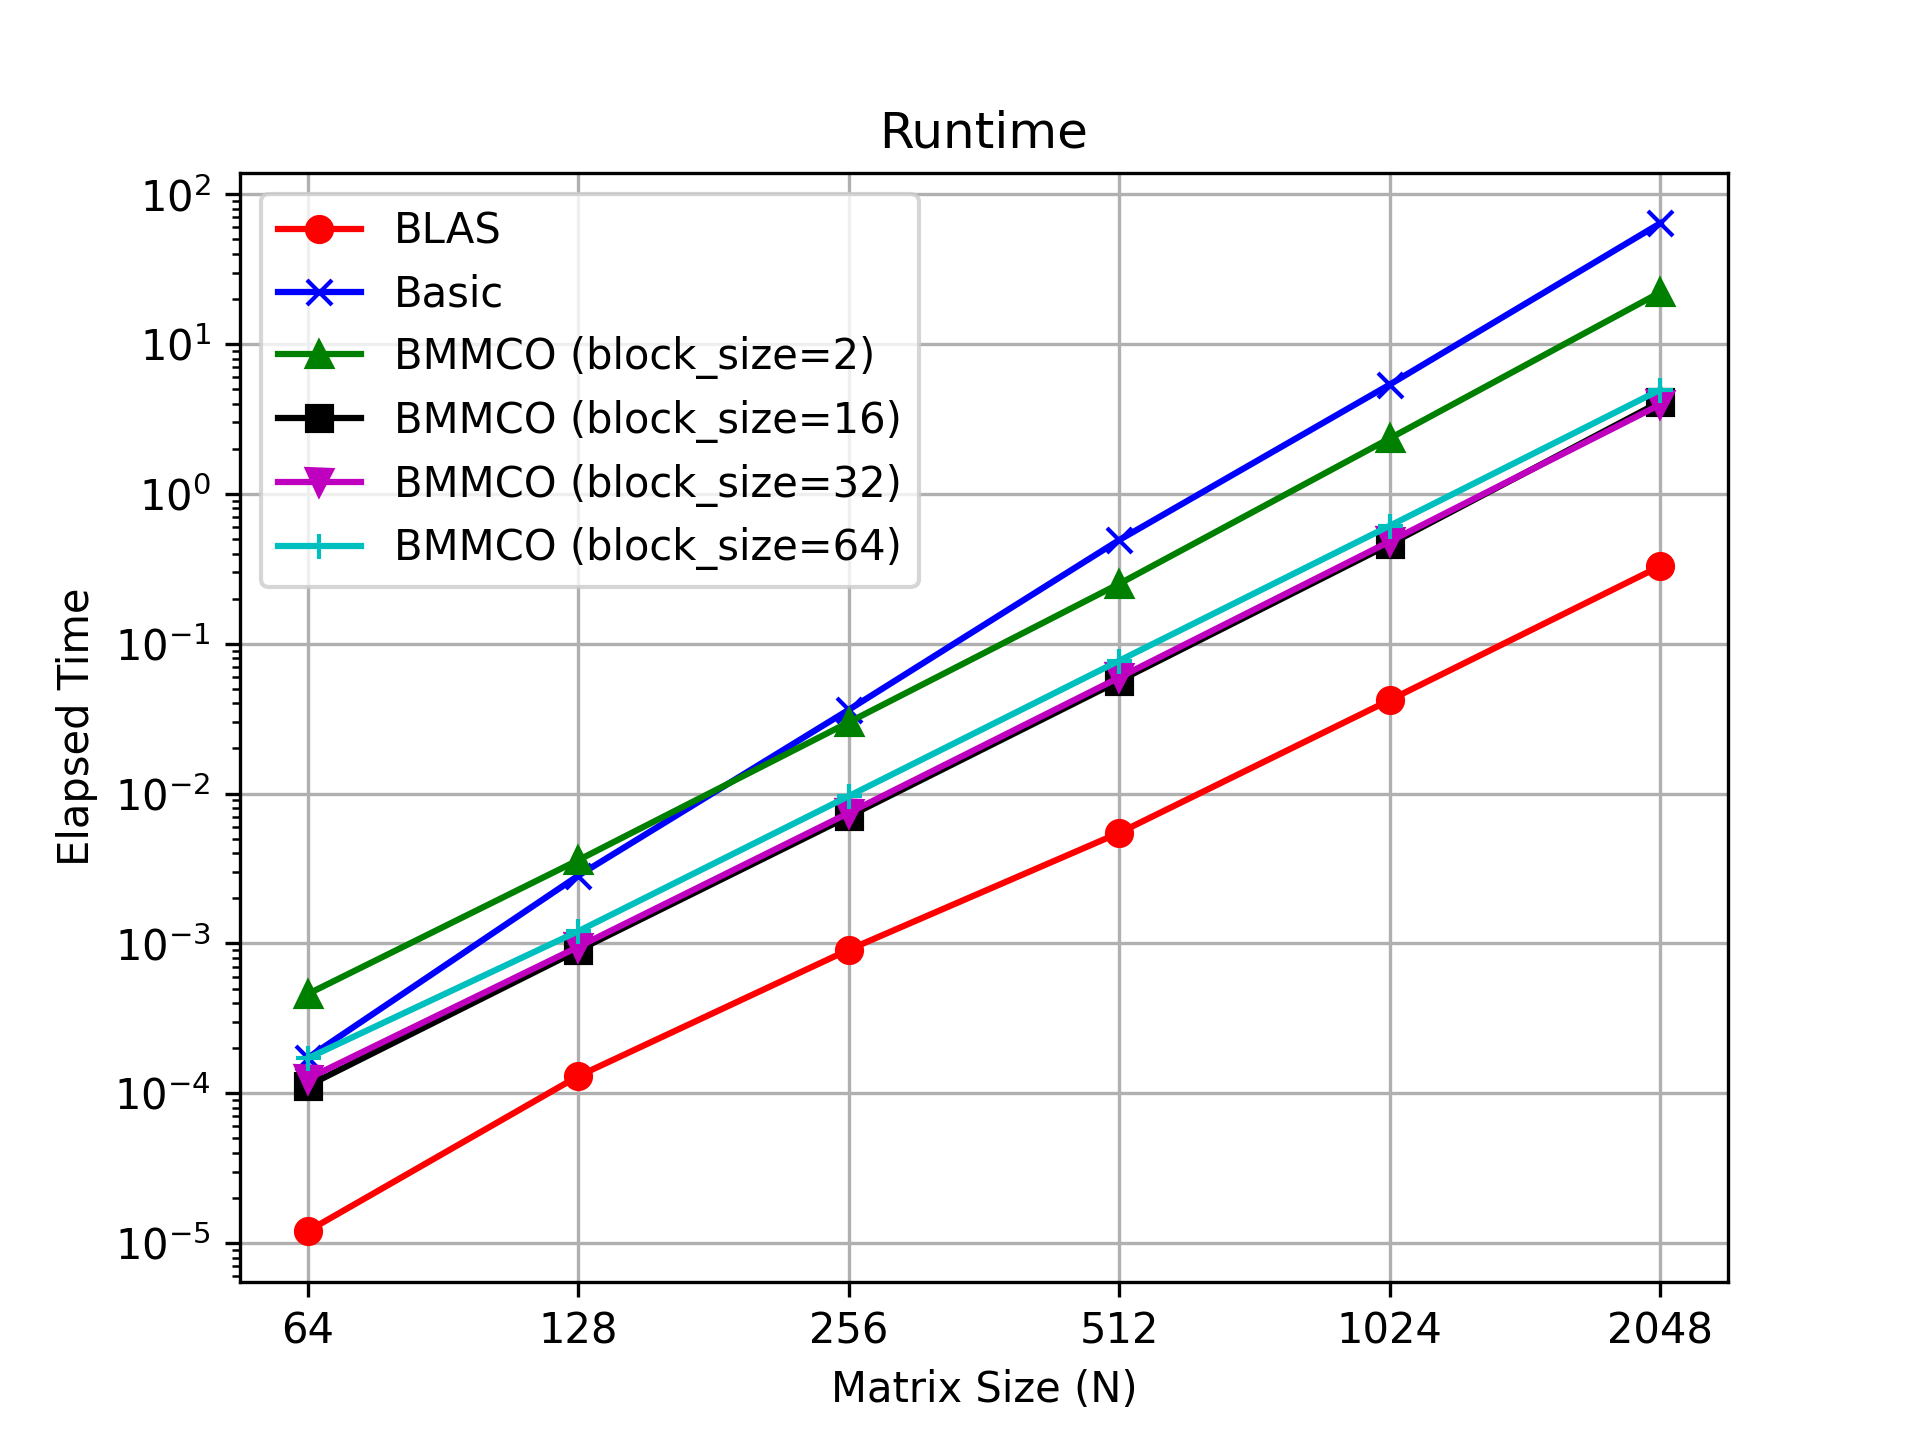
\includegraphics[width=1.0\linewidth]{images/Runtime.png}
%     \caption{Runtime comparison of all methods}
%     \label{fig:runtime}
% \end{figure}

\subsection{Comparison of Basic MM and CBLAS}
\label{subsec:basic-and-cblas}
\begin{comment}
    - Produce a chart comparing the performance of these two implementations across all problem sizes. The horizontal axis is problem size, the vertical axis is MFLOP/s (which you'll have to derive from runtime and your knowledge of the algorithm).
    - Discuss the performance of your Basic MM across the set of problem sizes. Do you see any changes of MFLOP/s across problem sizes? Describe the nature of those changes, if any, and provide an explanation of why the performance numbers change.
    - How does the performance of your Basic MM implementation compare to CBLAS, the reference implementation?
\end{comment}
% Describe the experiment in a few sentences: what question are you trying to answer, what problem sizes/etc did you use (it's ok to make reference back to Sec.~\ref{sec:methodology} so you don't have to repeat a lot of details. 

In this experiment, the objective is to establish a baseline for our evaluation by measuring the computational throughput (MFLOP/s) of Basic MM, an unoptimized implementation serving as our baseline, and CBLAS MM, a state-of-the-art, highly optimized implementation. The configuration details for this experiment are provided in Sec.~\ref{sec:methodology}.

As shown in Fig.~\ref{fig:mflops-Basic-CBLAS}, the MFLOP/s of the Basic MM decreases significantly as the problem size increases, while the MFLOP/s of the CBLAS implementation improves with larger matrix sizes. The decrease in Basic MM performance is almost inversely proportional to the matrix size, reflecting its inefficiency in terms of cache usage and memory access. In contrast, the CBLAS implementation shows a gradual improvement as the matrix size increases, with one exception: performance drops from \(64 \times 64\) to \(128 \times 128\). We believe this is caused by the initial discarded run for the \(64 \times 64\) problem size. It is likely that CBLAS’s \textit{cblas\_dgemm} method allocates an internal buffer based on the matrix size, which can be reused for efficiency in subsequent runs. The overhead of allocating this internal buffer is not negligible for smaller problem sizes, but the allocation process is skipped for \(64 \times 64\), leading to a performance drop for \(128 \times 128\).

Interestingly, the MFLOP/s of CBLAS sometimes exceeds the CPU core's theoretical peak performance of 39.2 GFLOP/s (see Sect.~\ref{sec:computeational-platform-and-software-environment}). During the execution, we verified that the program was not utilizing multiple cores by running the \textit{top} command, which showed a CPU usage value (\%CPU) close to, but less than, 100\%. We hypothesize that CBLAS is using advanced matrix multiplication techniques such as Strassen's algorithm, which can achieve a computational complexity better than \(O(N^3)\)\footnote{Strassen's algorithm has a complexity of approximately \(O(2^{2.8074})\).}. Therefore, our calculation of MFLOP/s using \(2N^3\) as \textit{ops} for CBLAS may not be entirely appropriate.

% Present the results of your experiment using either tabular forms of information, such as in Table~\ref{tab:MyTable1}, or using charts and graphs as in Fig.~\ref{fig:MyPlot1}.
\begin{figure}[htbp]
    \centering
    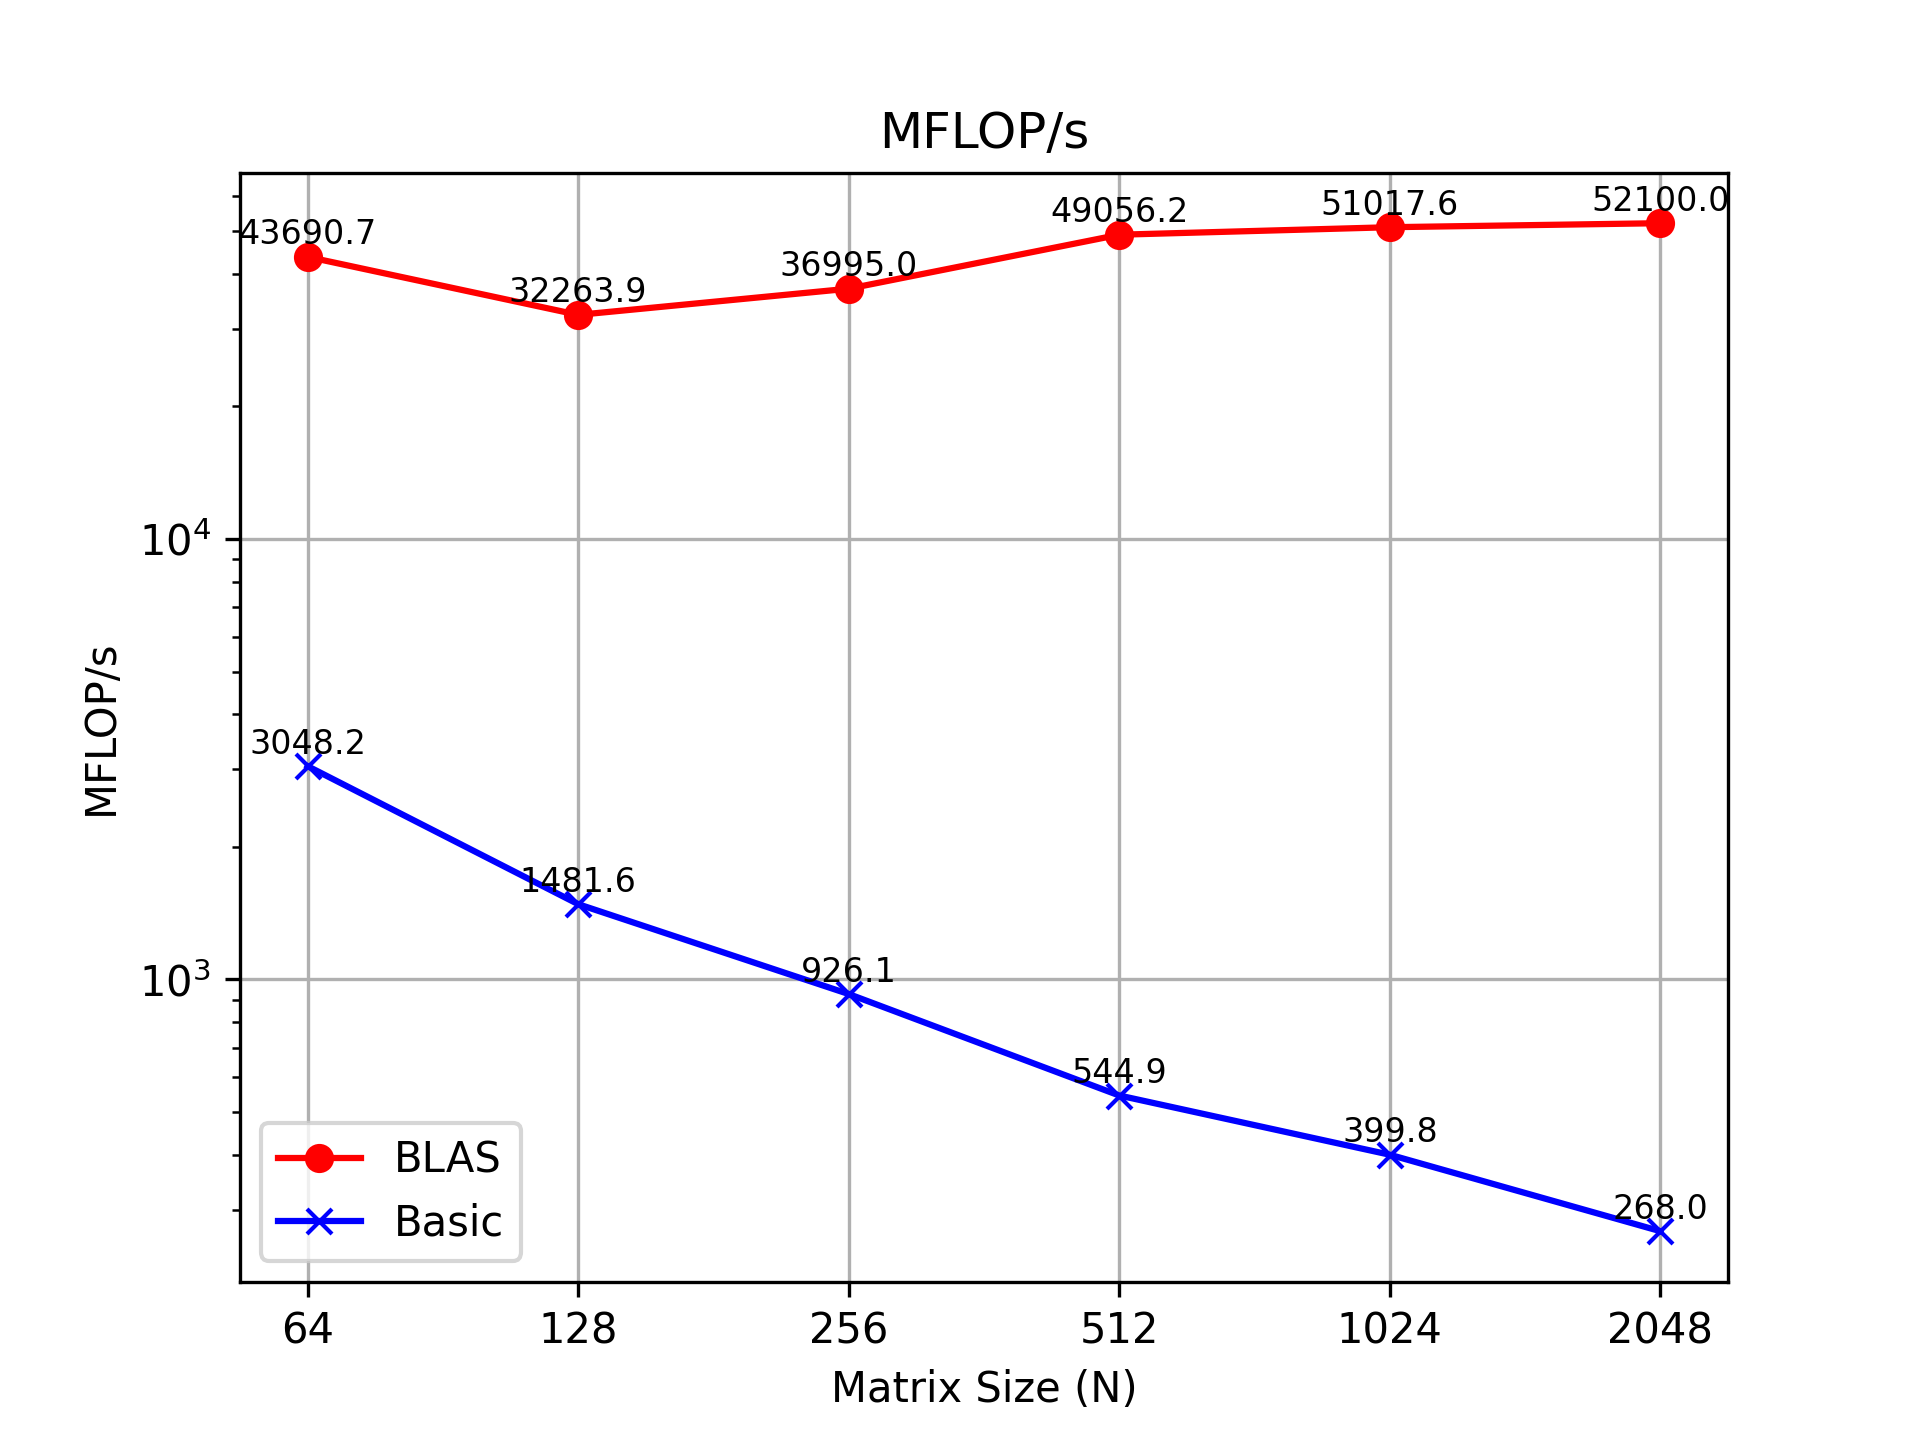
\includegraphics[width=1.0\linewidth]{images/Basic-MM-and-CBLAS_MFLOPs.png}
    \caption{\textbf{MFLOP/s comparison of Basic MM and CBLAS MM across different matrix sizes.} The matrix is \(N \times N\). Note that MFLOP/s decreases consistently on a logarithmic scale for Basic MM as the matrix size increases. In contrast, MFLOP/s gradually increases for CBLAS MM, with the exception of a performance drop from \(64 \times 64\) to \(128 \times 128\). This drop is likely due to the initial discarded run for the \(64 \times 64\) problem size.}
    \label{fig:mflops-Basic-CBLAS}
\end{figure}

\subsection{Blocked MM with Copy Optimization (BMMCO), and CBLAS}
\label{subsec:bmmco-and-cblas}

In this experiment, we evaluate the efficiency of the BMMCO implementation at four different block sizes by comparing its MFLOP/s with that of the CBLAS implementation. The configuration details for this experiment are provided in Sec.~\ref{sec:methodology}. Figure~\ref{fig:mflops-BMMCO-CBLAS} shows how block size and matrix size affect the MFLOP/s of BMMCO compared to the CBLAS MM implementation. From this figure, three key insights can be derived.

\begin{figure}[htbp]
    \centering
    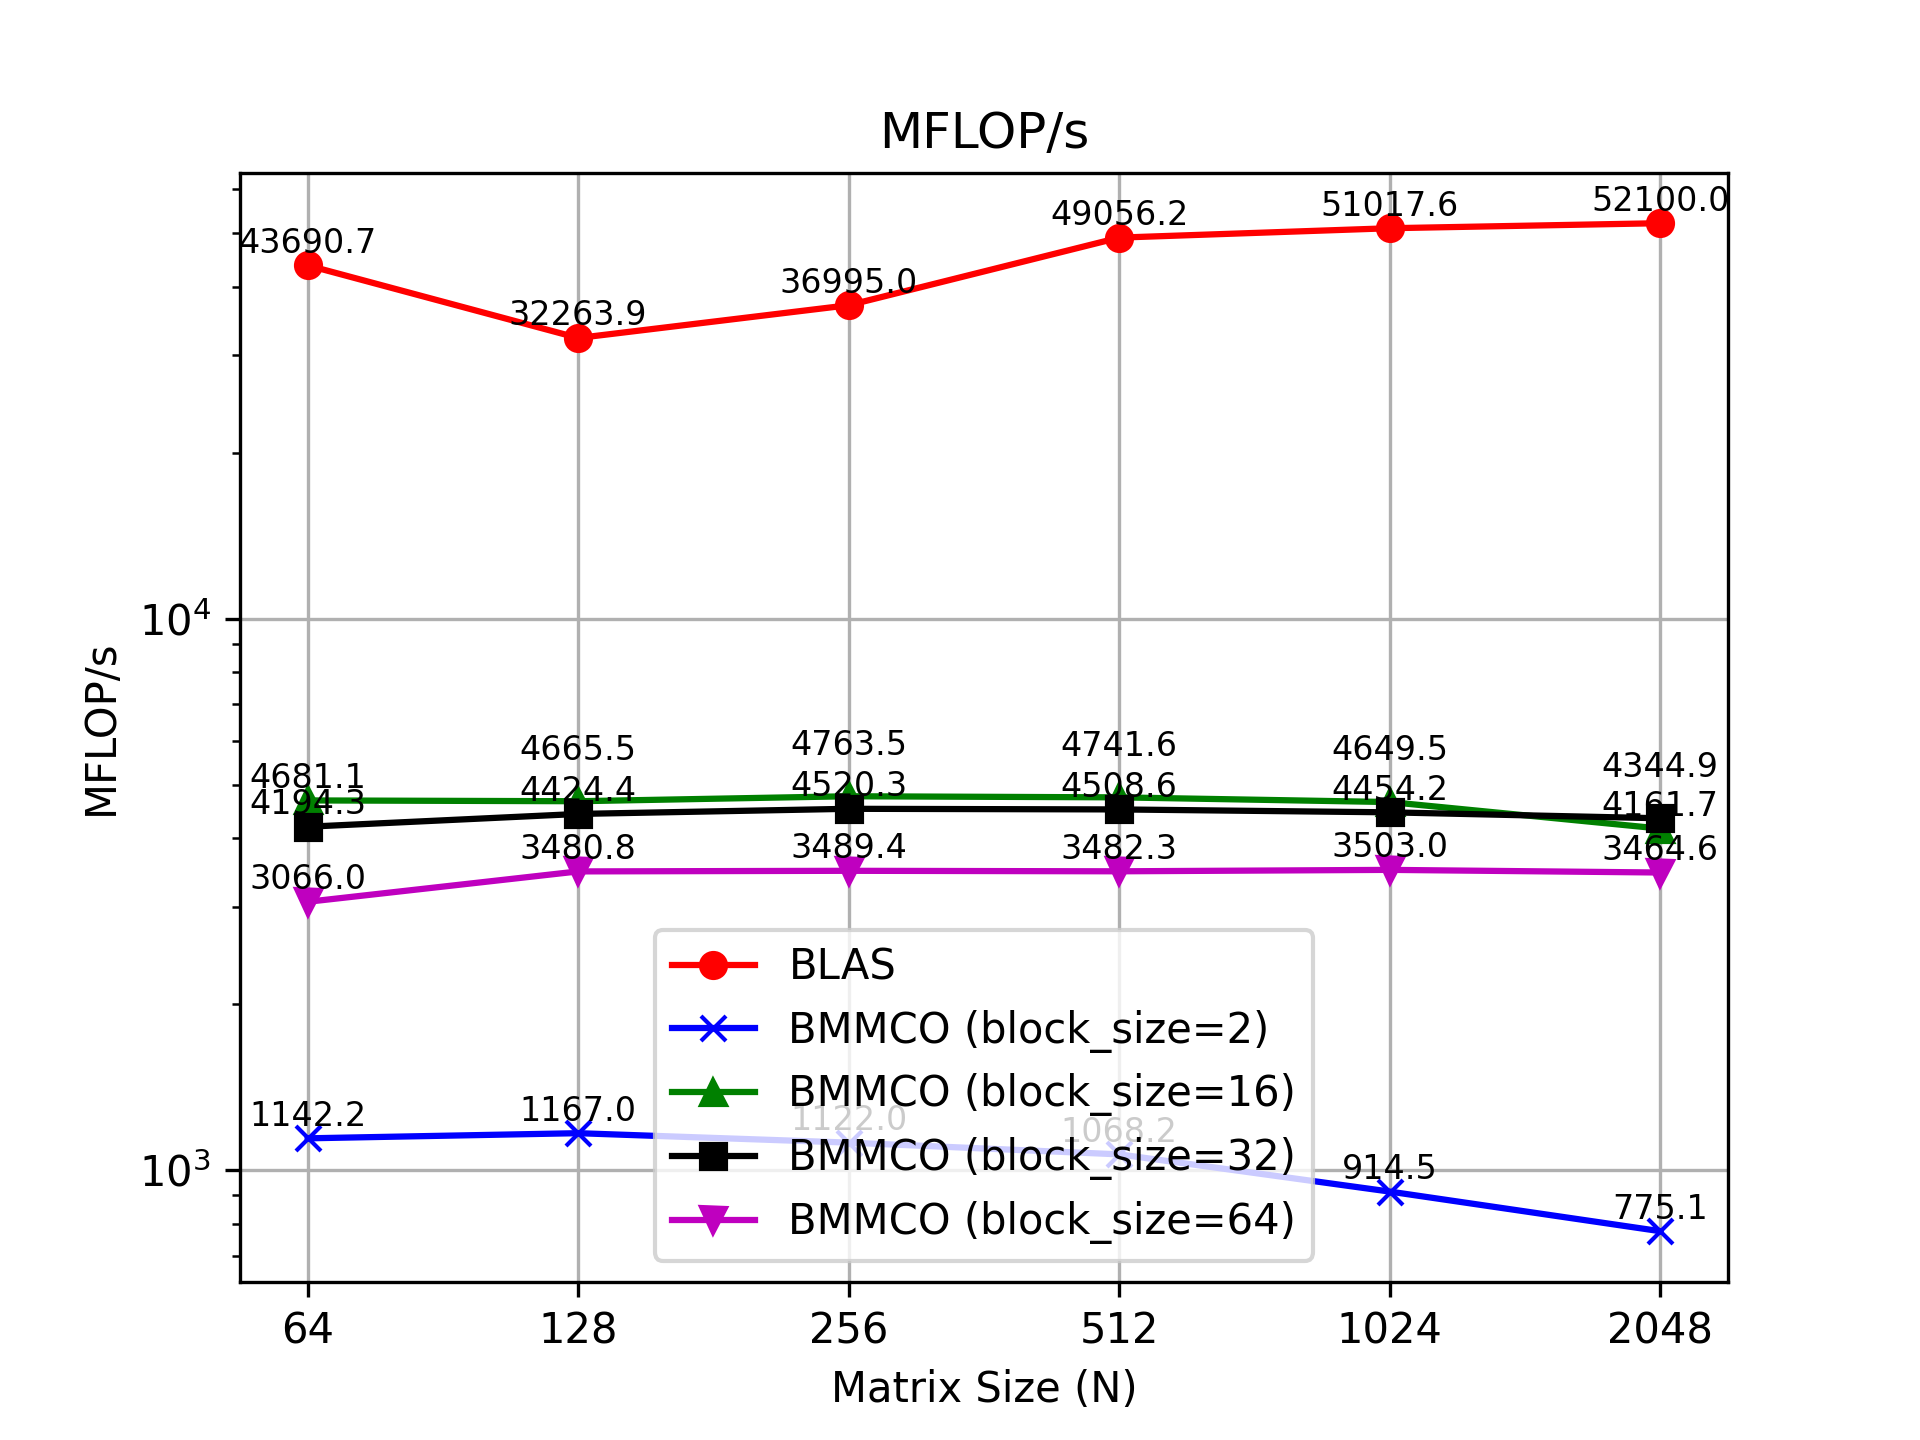
\includegraphics[width=1.0\linewidth]{images/BMMCO-and-CBLAS_MFLOPs.png}
    \caption{\textbf{MFLOP/s comparison of BMMCO and CBLAS MM across different block sizes and matrix sizes.} The matrix is \(N \times N\). The figure illustrates how BMMCO's performance varies with block sizes of 2, 16, 32, and 64, compared to the highly optimized CBLAS MM implementation. The block size of 2 is significantly inefficient due to the limited performance gain from small block sizes. While larger block sizes generally improve performance, the block size of 64 shows performance degradation due to exceeding the L1 cache capacity, as discussed in Sec.~\ref{subsubsec:l1-cache-fit}.}
    \label{fig:mflops-BMMCO-CBLAS}
\end{figure}

\subsubsection{Performance limitation of small block sizes}
\label{subsubsec:blocking-overhead}
The first insight is that the block size of 2 is significantly inefficient compared to larger block sizes, and its MFLOP/s decreases as the matrix size increases, following a similar trend to the Basic MM implementation in Section~\ref{subsec:basic-and-cblas}. This inefficiency is due to the fact that the performance gain is primarily limited by the small block size\footnote{The number of slow memory operations, \(m\), depends on the block size \(b\) and the matrix size \(N\). The total number of slow memory operations is proportional to \((2N_b + 2) \cdot N^2\), where \(N_b\) is the number of blocks. Compute intensity (CI), defined as \(CI = \frac{\textit{ops}}{\textit{number of slow memory accesses}}\), improves with larger block sizes as CI approaches \(n/N_b = b\) for large matrices.}.

\subsubsection{Impact of L1 cache capacity on performance}
\label{subsubsec:l1-cache-fit}
The second insight is that larger block sizes, particularly 16 and 32, perform better. The block size of 16 produced the best results, while the block size of 32 performed slightly worse. However, the block size of 64 showed a performance degradation of approximately 20-30\% compared to both 16 and 32. Initially, we expected larger block sizes to consistently provide better MFLOP/s, so these results were counterintuitive. This discrepancy is due to L1 cache utilization. As shown in Table~\ref{tab:memory-footprint-three-blocks-l1-cache}, the block size of 64 requires a memory footprint of 96 KiB for three blocks, which exceeds the 32 KiB L1 cache capacity (see Sec.~\ref{sec:computeational-platform-and-software-environment}). While block sizes up to \(32 \times 32\) fit within the L1 cache, the block size of 64 does not, resulting in performance degradation as tiling and blocking optimizations rely on fitting blocks into fast memory.

\begin{table}[htbp]
    \centering
    \begin{tabular}{c|c|c}
        \textbf{Block Size} & \textbf{3 Blocks (Bytes)} & \textbf{L1 Cache Fit} \\
        \hline
        \(2 \times 2\) & 96 B & Yes \\
        \(16 \times 16\)  & 6 KiB & Yes \\
        \(32 \times 32\)  & 24 KiB & Yes \\
        \(64 \times 64\)  & 96 KiB & No \\
    \end{tabular}
    \caption{\textbf{Memory footprint for different block sizes and L1 cache fit.} The table shows the memory required for three blocks of each size and whether they fit within the L1 cache (32 KiB). Block sizes up to \(32 \times 32\) fit, while \(64 \times 64\) does not.}
    \label{tab:memory-footprint-three-blocks-l1-cache}
\end{table}

\subsubsection{Remaining Performance Gap Between BMMCO and CBLAS}
\label{subsubsec:remaining-performance-gap-between-bmmco-cblas}
Even with the best BMMCO results (block size of 16), the CBLAS MM implementation still outperforms BMMCO by approximately tenfold. This significant performance gap suggests that there is still room for optimization, such as loop reordering, improved in-memory data layout strategies, and the use of advanced matrix multiplication algorithms like Strassen's algorithm.


\subsection{Findings and Discussion}
\label{subsec:findings-and-discussion}
\begin{comment}
    - Compare the differences between basic MM, blocked MM with copy: what differences and similarities do you see between the basic and blocked versions?
    - In places where one outperforms others, discuss why you believe that to be the case?  Does that correspond to any features of the hardware you are using?
    - Looking at all the datasets, do you see any changes of performance across problem sizes?
    - Describe the nature of those changes, if any, and provide an explanation of why the performance numbers change.
\end{comment}
From Figure\ref{fig:mflops-BMMCO-Basic}, we can gain two key insights.

\begin{figure}
    \centering
    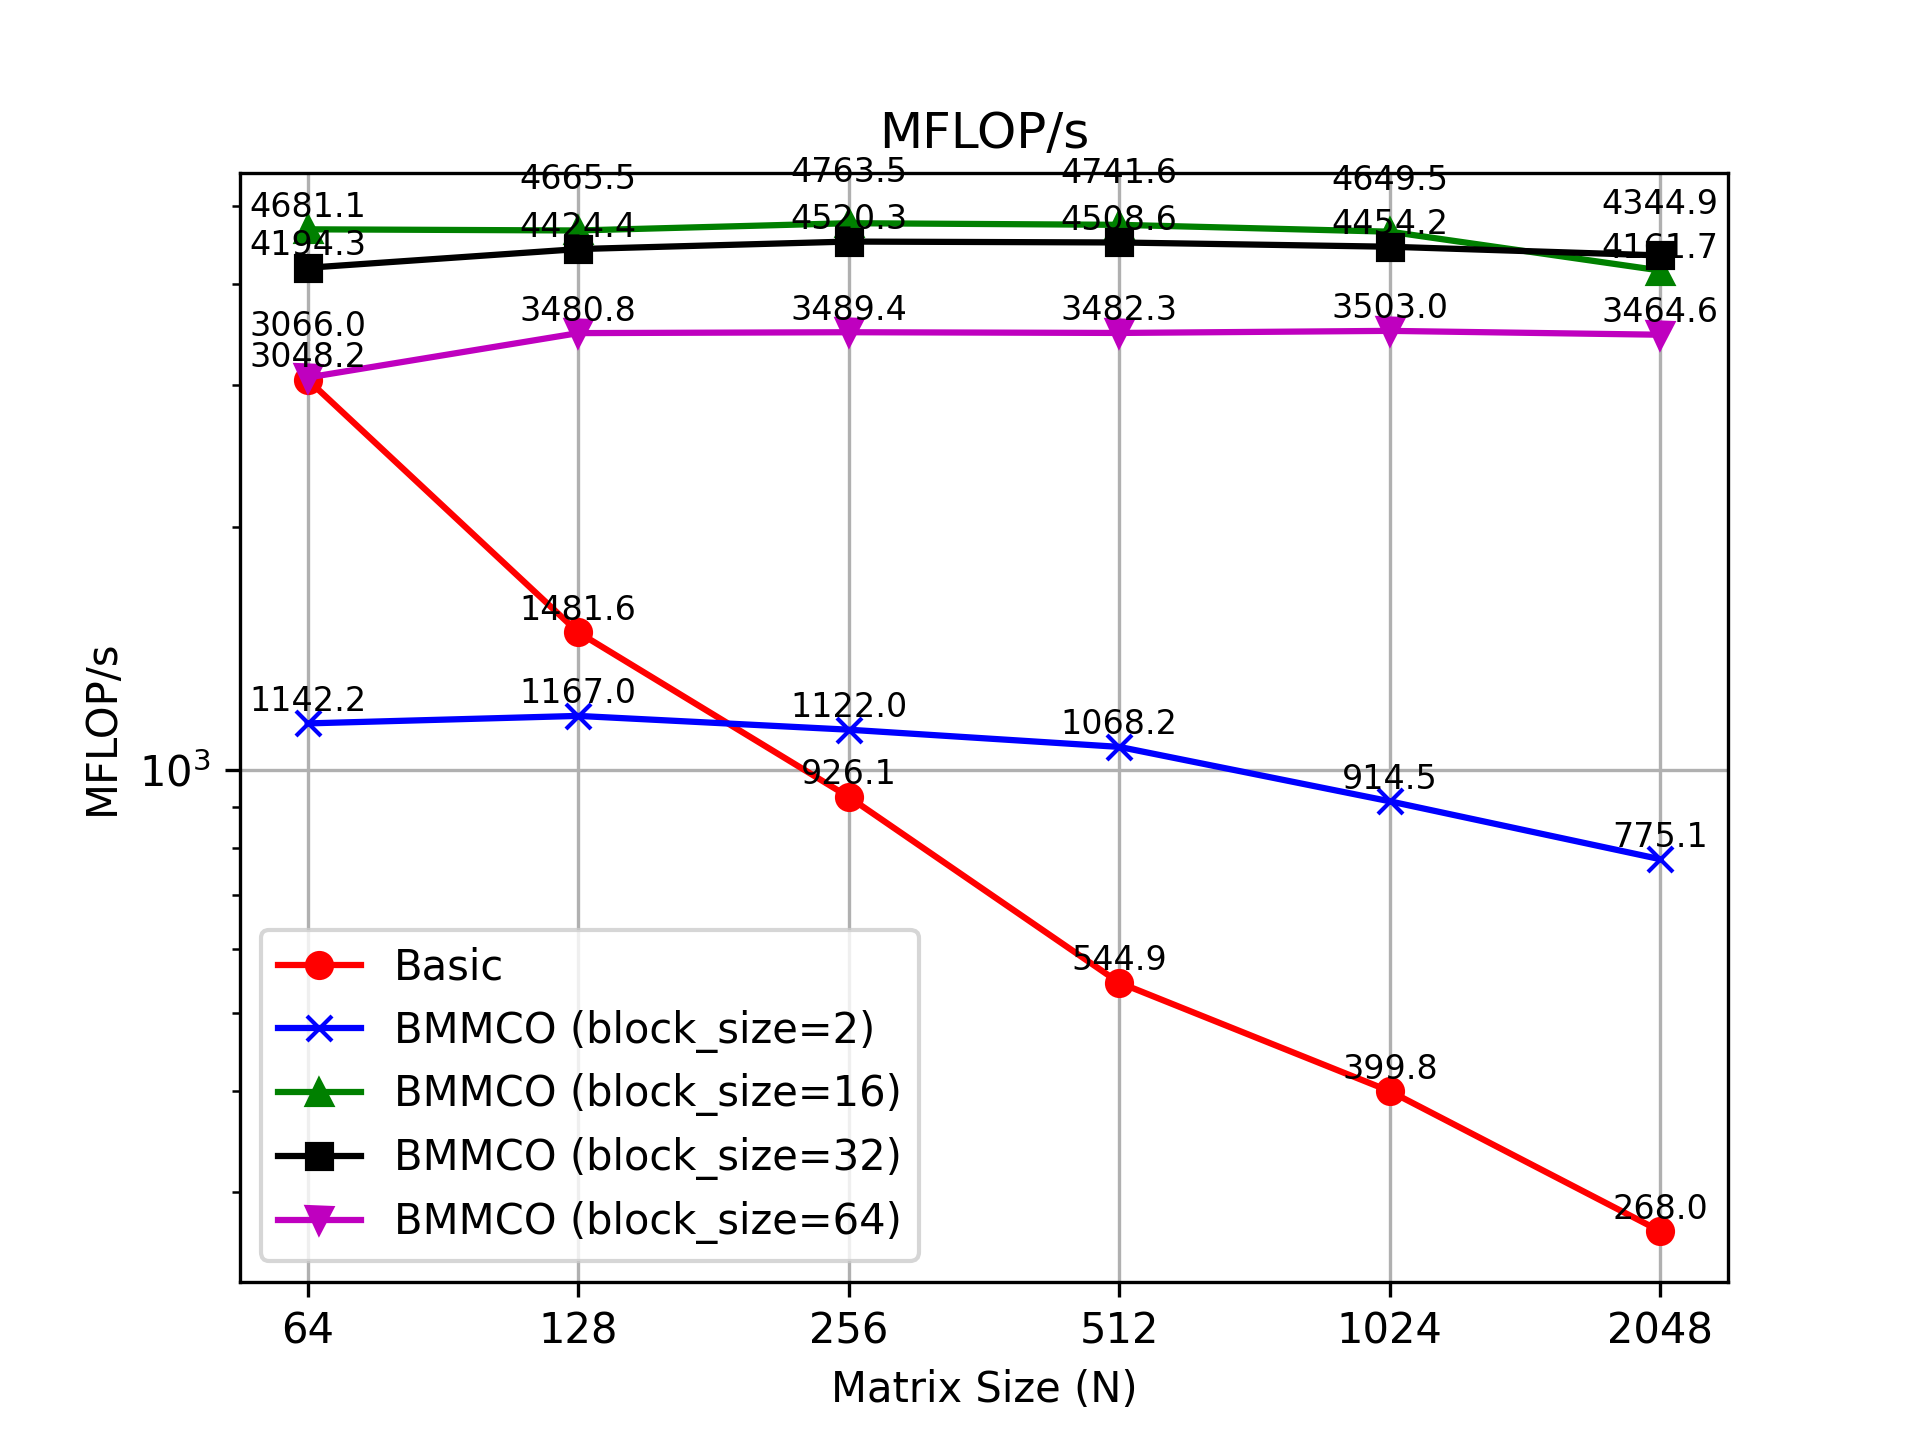
\includegraphics[width=1.0\linewidth]{images/BMMCO-and-Basic_MFLOPs.png}
    \caption{\textbf{MFLOP/s Comparison of BMMCO and Basic MM across Matrix Sizes.} This figure illustrates the performance differences between BMMCO and Basic MM across various matrix sizes. BMMCO shows more stable performance with larger matrix sizes due to optimization techniques such as blocking and copy, while Basic MM's performance degrades as the matrix size increases.}
    \label{fig:mflops-BMMCO-Basic}
\end{figure}

\FloatBarrier
\subsubsection{Poor performance of BMMCO with a block size of 2}
\label{subsubsec:poor-performance-bmmco-block-size-2}
The BMMCO implementation with a block size of 2 exhibits significantly lower performance than Basic MM for matrix sizes of \(64 \times 64\) and \(128 \times 128\). This can be attributed to the fact that matrices A, B, and C all fit entirely within the 512 KiB L2 cache, with a significant portion of them also fitting into the 32 KiB L1 cache for these sizes (see Table~\ref{tab:memory-footprint-three-matrices}). As a result, the benefits of blocking and copy optimization are outweighed by the overhead introduced (i.e., reading and writing blocks to internal buffer).

The MFLOP/s of BMMCO with a block size of 2 decreases as the problem size increases, following a similar trend observed in Basic MM, though the decline is more gradual. This is because, for larger matrix sizes that do not fit into the L2 cache, the overhead becomes relatively smaller, and the gains from optimization become more substantial.

\begin{table}[htbp]
    \centering\small
    \begin{tabular}{c|c|c|c|c}
        \textbf{Matrix Size} & \textbf{3 Matrices (Bytes)} & \textbf{L1} & \textbf{L2} & \textbf{L3} \\
        \hline
        \(64 \times 64\) & 96 KiB & No & Yes & Yes \\
        \(128 \times 128\) & 384 KiB & No & Yes & Yes \\
        \(256 \times 256\) & 1.5 MiB & No & No & Yes \\
        \(512 \times 512\) & 6 MiB & No & No & Yes \\
        \(1024 \times 1024\) & 24 MiB & No & No & Yes \\
        \(2048 \times 2048\) & 96 MiB & No & No & No \\
    \end{tabular}
    \caption{\textbf{Memory footprint for different matrix sizes and cache fit.} The table shows the memory footprint required to hold three matrices of varying sizes and whether they fit within the L1 cache (32 KiB), L2 cache (512 KiB), and L3 cache (32 MiB). Matrices up to \(128 \times 128\) fit in the L2 cache, and those up to \(512 \times 512\) fit within the L3 cache.}
    \label{tab:memory-footprint-three-matrices}
\end{table}

\subsubsection{Large Block Sizes Outperform Basic MM}
\label{large-block-outperform-basic}

For a matrix size of \(64 \times 64\), the performance of Basic MM is comparable to that of BMMCO with a block size of 64. This is because the matrix size and block size are equal, resulting in no significant performance gain from the BMMCO implementation.

However, BMMCO with larger block sizes consistently outperforms Basic MM, with performance remaining relatively stable across different matrix sizes, while Basic MM’s MFLOP/s decreases almost inversely as the matrix size increases. This improvement in BMMCO is due to performance gains that scale with the block size (see the footnote\footnotemark[3]) when the blocks fit into fast memory. In fact, the three blocks used in the optimization mostly fit within the L1 cache and fully fit within the L2 cache (see Table~\ref{tab:memory-footprint-three-blocks-l1-l2-cache}), allowing matrix multiplication to proceed with minimal slow memory access, thereby increasing efficiency.

In summary, without blocking and copy optimization, performance degrades significantly due to inefficient memory access. However, by leveraging these optimizations, both spatial and temporal locality are effectively utilized, leading to substantial improvements in overall efficiency.

\begin{table}[htbp]
    \centering
    \begin{tabular}{c|c|c|c}
    \textbf{Block Size} & \textbf{3 Blocks (Bytes)} & \textbf{L1 Cache} & \textbf{L2 Cache} \\
    \hline
    \(2 \times 2\) & 96 B & Yes & Yes \\
    \(16 \times 16\) & 6 KiB & Yes & Yes \\
    \(32 \times 32\) & 24 KiB & Yes & Yes \\
    \(64 \times 64\) & 96 KiB & No & Yes \\
    \end{tabular}
    \caption{\textbf{Memory Footprint for different block sizes  and L1 and L2 cache fit.} This table shows the memory footprint required to hold three blocks of different sizes and whether they fit within the L1 and L2 cache levels. Block sizes up to \(32 \times 32\) fit within the L1 cache, while larger block sizes fit within the L2 cache.}
    \label{tab:memory-footprint-three-blocks-l1-l2-cache}
\end{table}

% \begin{table}[htbp]
%     \centering
%     \begin{tabular}{c|c|c|c|c}
%     N & footprint & L1(32KB) & L2(512KB) & L3(32MB) \\
%     \hline
%     64 & 32KB & x & O & O \\
%     128 & 128KB & x & O & O \\
%     256 & 512KB & x & O & O \\
%     512 & 2MB & x & x & O \\
%     1024 & 8MB & x & x & O \\
%     2048 & 32MB & x & x & O \\
%     \end{tabular}
%     \caption{Memory footprint to hold single matrix}
%     \label{tab:memory-footprint-single-matrix}
% \end{table}

% Also, optionally include any additional insights you gained while doing these performance experiments.

% If this were an actual tech paper, here is where you would summarize the main findings and observations from the experiments: do the experiment results support your hypothesis? Sometimes the answer is a clear Y. Sometimes, the answer is Y for some circumstances, but not all, and it is important to spell this out.

% Sometimes, the experiments turn up unexpected negative results, and it is also important to point out those, as well. Science happens due to both successes and failures, and it is important to document failed experiments so that we can all learn from them.
\section{Conclusions and Future Work}
\label{sec:conclusion-and-future-work}

As we saw in the memory usage, our current implementation has extra implementation overhead of memory usage, potentially affecting the overall performance. So we want to improve the code to replace complex classes to Plain Old Data (POD), such as arrays and structs. This has another benefit such as enabling the OpenMP GPU offloading.

Our current implementation only supports spheres as the object type, but we aim to extend this to support planes and polygons at a minimum. Expanding the range of supported primitives would enable more realistic and complex scenes to be rendered, enhancing the utility of our ray tracing system.

Additionally, we plan to evaluate the performance of our implementation by comparing it against OptiX\cite{nvidia_optix}, a state-of-the-art GPU ray tracing framework, which would provide a highly optimized baseline. Such a comparison would help identify specific bottlenecks in our implementation and validate the scalability and efficiency of our parallelization strategies.

Finally, while our work demonstrates the potential of parallelism for ray tracing, achieving real-time performance remains a significant challenge. In the future, we aim to explore advanced optimization techniques such as hierarchical acceleration structures and adaptive sampling to push the boundaries of performance further. These improvements could bring us closer to real-time applications in gaming and visualization.



%% if specified like this the section will be committed in review mode
\acknowledgments{
This paper was edited with the assistance of \textit{ChatGPT (GPT-4o, GPT-o1, GPT-o1-mini, and GPT-o1 pro mode)} (accessed December 2024), primarily for correcting grammatical errors, rephrasing, and addressing technical queries as a substitute for search engines. This research was supported by resources from the National Energy Research Scientific Computing Center (NERSC), a Department of Energy Office of Science User Facility, under NERSC award DDR-ERCAP m3930 for 2024.
}

\bibliographystyle{abbrv-doi}

% uncomment the following line if you decide to include a bibliography (references) with your homework writeup
\bibliography{template}

\appendix
\appendixpage
\section{Sample Images Generated by Our Ray Tracing Program}

This section showcases sample images generated using our ray tracing program. These images demonstrate the program's capabilities and highlight the effects of varying parameters such as scene complexity, rendering resolution, and threading configurations.

\begin{figure}[htbp]
    \centering
    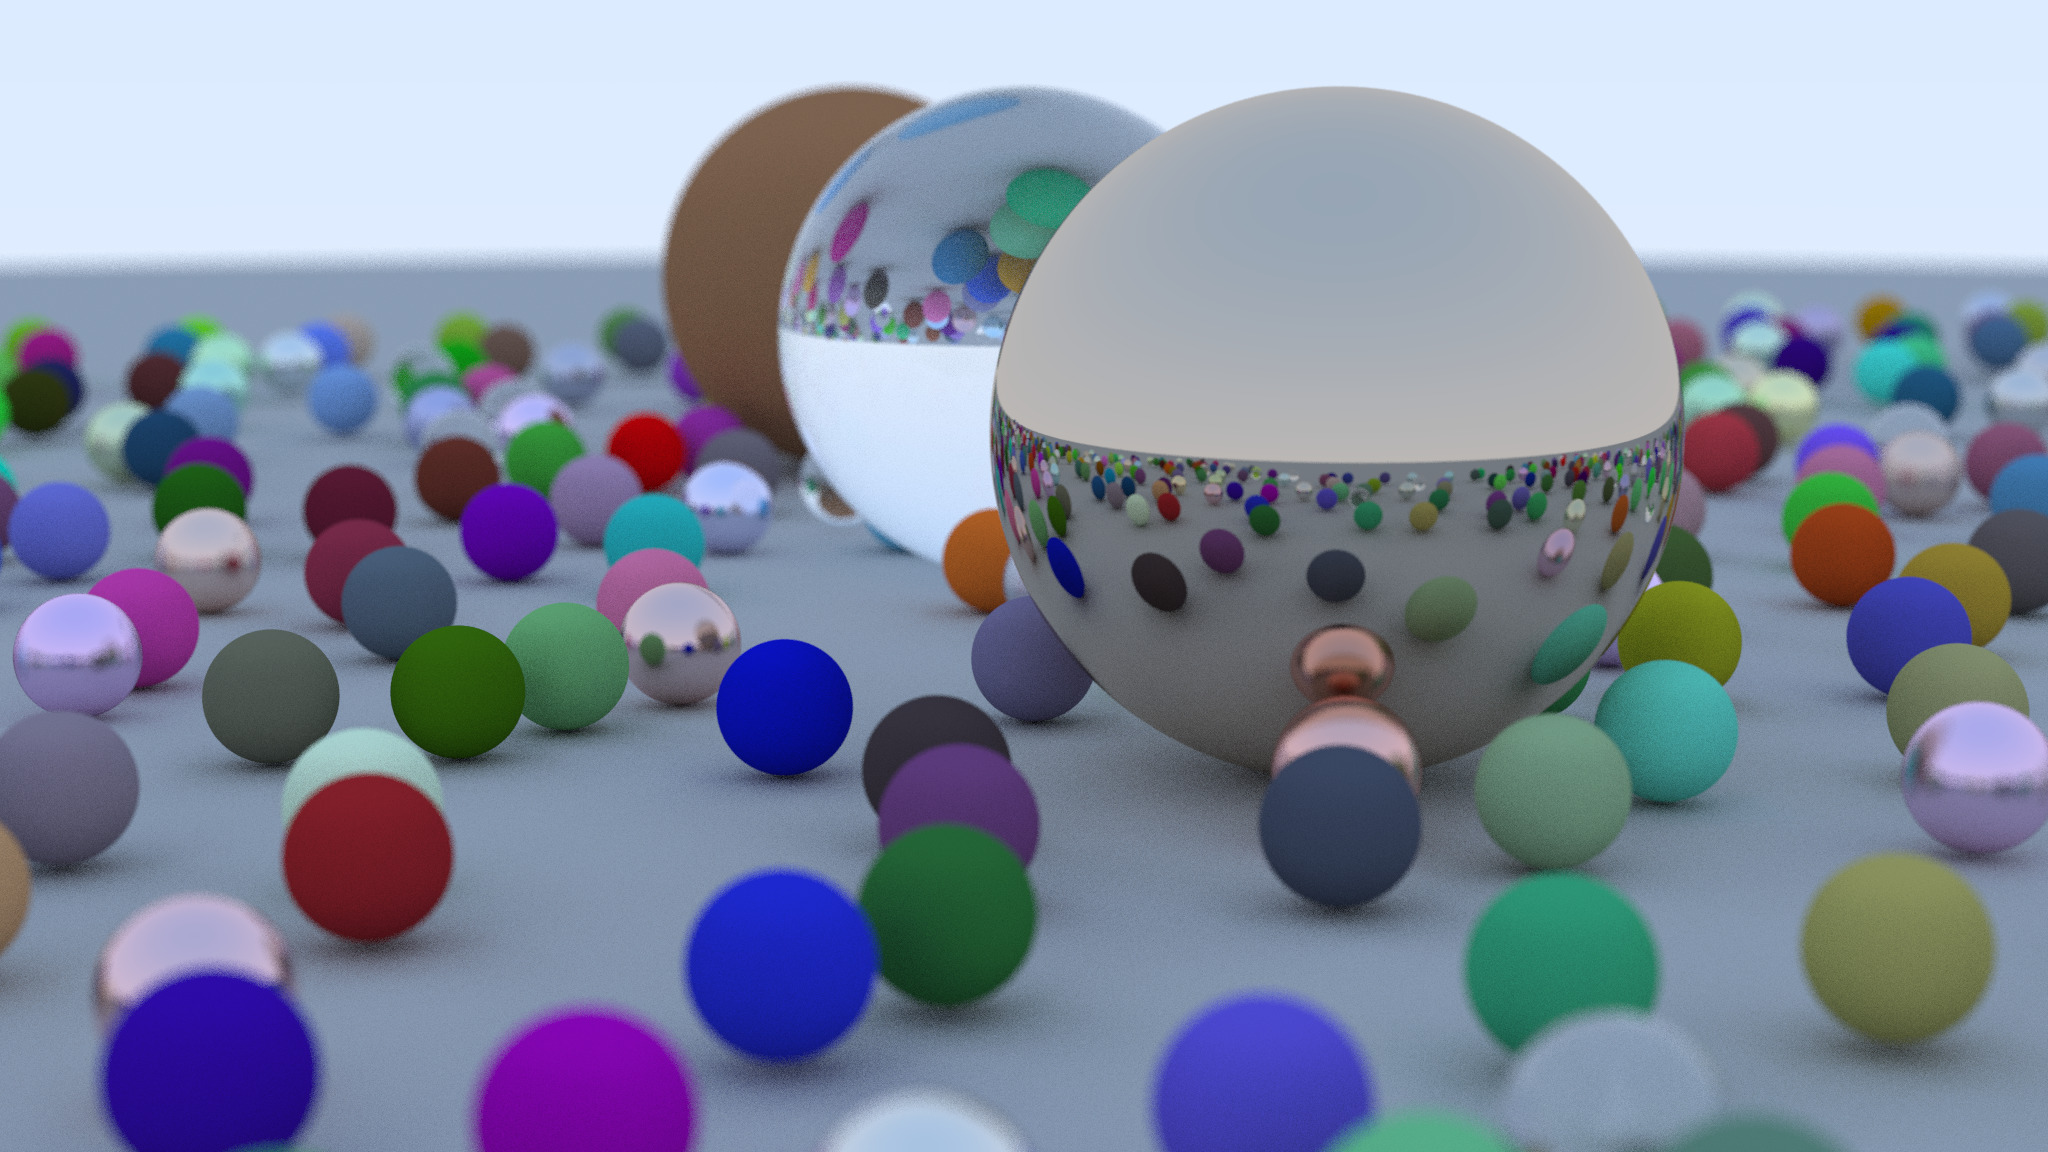
\includegraphics[width=1.0\linewidth]{images/fine-image.jpg}
    \caption{A high-quality image rendered with the following parameters: Samples per pixel = 32, Width = 2048, Height = 1152, Max Recursion Depth = 32, Scene Complexity = 11, Threads = 8, Schedule = Static. This example highlights the program's ability to handle complex scenes and produce detailed, photorealistic output.}
    \label{fig:sample-image-fine}
\end{figure}

The following figure compares scene complexity across three different configurations. Scene complexity determines the number of objects in the scene, which directly impacts rendering time and the level of detail in the output. A higher scene complexity results in more objects being rendered, creating a richer visual but also increasing computational demands.

\begin{figure}[htbp]
  \centering
  \begin{minipage}{0.3\textwidth}
    \centering
    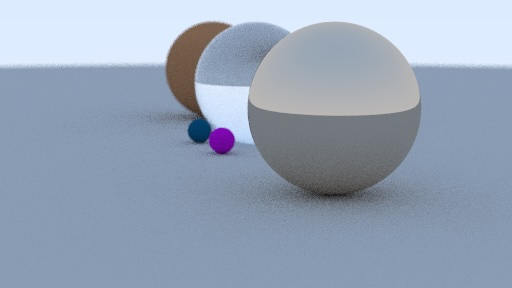
\includegraphics[width=\linewidth]{images/image-sphere-grid-1.jpeg}
    \subcaption{Scene Complexity = 1}
  \end{minipage}
  \begin{minipage}{0.3\textwidth}
    \centering
    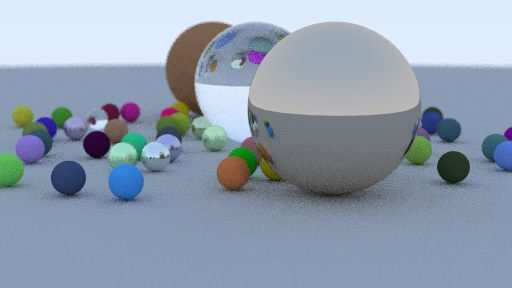
\includegraphics[width=\linewidth]{images/image-sphere-grid-4.jpeg}
    \subcaption{Scene Complexity = 4}
  \end{minipage}
  \begin{minipage}{0.3\textwidth}
    \centering
    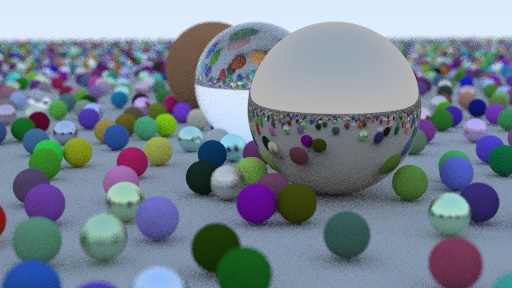
\includegraphics[width=\linewidth]{images/image-sphere-grid-64.jpeg}
    \subcaption{Scene Complexity = 64}
  \end{minipage}
  \caption{Illustration of scene complexity: (a) Scene Complexity = 1, (b) Scene Complexity = 4, (c) Scene Complexity = 64. As the complexity increases, the number of spheres in the grid grows, creating a more detailed and computationally intensive scene.}
  \label{fig:three_sphere_grids}
\end{figure}

\FloatBarrier
\section{Runtime Memory Footprint Investigation}
\label{sec:memory-footprint}

The memory footprint associated with different scene complexities, calculated at runtime, is shown in Table~\ref{tab:memory-footprint}. Each iteration (sampling a color for a ray) requires approximately 400 bytes per object for intersection testing in the current implementation. However, a detailed breakdown of the actual data needed for a single object reveals significant inefficiencies in memory usage. Optimizing the memory usage by minimizing overhead or restructuring data could dramatically reduce the memory footprint, leading to enhanced performance for large-scale scenes.

\begin{table}[htbp]
    \centering
    \small
    \begin{tabular}{|c|c|c|}
        \hline
        \textbf{Scene Complexity} & \textbf{Number of Small Spheres} & \textbf{Memory Footprint (KiB)} \\
        \hline
        1  & 4       & 1.5    \\
        16 & 1024    & 201    \\
        64 & 16384   & 3,276  \\
        \hline
    \end{tabular}
    \caption{Runtime Memory Footprint for the \texttt{world} at Different Scene Complexities.}
    \label{tab:memory-footprint}
\end{table}

\subsection{Minimum Memory Requirements for an Object}

The theoretical minimum size for a single object, based on the attributes used in intersection testing, is calculated as follows:
\begin{itemize}
    \item \textbf{Center coordinates:} 24 bytes (3 double-precision values)
    \item \textbf{Radius:} 8 bytes (1 double-precision value)
    \item \textbf{Material type:} 0.25 bytes (2-bit value, rounded for calculation)
    \item \textbf{Albedo:} 24 bytes (3 double-precision values)
    \item \textbf{Fuzz:} 8 bytes (1 double-precision value)
    \item \textbf{Refraction index:} 8 bytes (1 double-precision value)
    \item \textbf{Total Minimum Size:} 72.25 bytes
\end{itemize}

Considering hardware and compiler constraints, such as memory alignment or padding, this size may round up to the nearest memory block boundary, typically 8 or 16 bytes. This results in a practical memory usage of approximately 80 bytes per object.

\end{document}
